\chapter[本模板简单的使用说明]{本模板简单的使用说明\protect\footnote{本章由ywg添加}}
\section{模板基本信息}
\subsection{模板简介}
本模板是按照中国科学技术大学教务处规定制作的,适合于本科生毕业论文撰写的\LaTeX 模板,模板在ctexbook文档类的基础上进行了修改,添加了一些常用的宏包和命令。

\subsection{提出疑问及报告Bug}
如果您在使用过程中有疑问,遇到困难,可以在\href{http://bbs.ustc.edu.cn/cgi/bbsdoc?board=TeX}{瀚海星云\TeX{}讨论区}或者相关的\LaTeX 论坛(如\href{http://bbs.ctex.org}{CTEX 论坛})寻求帮助,但是请注意遵守论坛的各项规定。

如果使用过程中遇到Bug,请提交到\href{http://bbs.ustc.edu.cn/cgi/bbsdoc?board=TeX}{瀚海星云\TeX{}讨论区},或者提交到相应的\href{http://code.google.com/p/ustcthesis/issues/list}{Google UstcThesis Project(http://code.google.com/p/ustcthesis/issues/list)},请注明是本科论文模板的bug。

\subsection{如何得到本模板}
可以在\href{http://code.google.com/p/ustcthesis/downloads/list}{Google UstcThesis Project(http://code.google.com/p/ustcthesis/downloads/list)}下载到完整的模板文件(包括本说明文档)。

\section{模板基本设置}
使用本模板,您应首先具备基本的\LaTeX 知识,如果您刚刚接触\LaTeX,建议您先学习相关的用户文档或教程。

模板文件名为ustcthesis.cls。方便起见,将该文件放置在与论文主文件同一文件夹中即可。

模板提供一个文档类ustcthesis,使用\verb|\documentclass{ustcthesis}|来加载模板。

模板可以使用ctexbook文档类的相应选项,默认加载的是 12pt, a4paper, fancyhdr, fntef, twoside, opentight。需要注意的是默认加载 \emph{双面/章节从奇数页开始} 选项,如果需要\emph{单面} 选项,请使用:\begin{center}\verb|\documentclass[oneside,openany]{ustcthesis}|\end{center}

模板提供了两个新的文档选项 capnocolon 和 titlechinese,它们具体的效果如下:
\begin{description}
\item[capnocolon]{去掉图表标题序号中的“:”(\autoref{pic:capnocolon})}
\item[titlechinese]{章节标题使用中文格式(\autoref{pic:titlech})}
\end{description}

\begin{figure}
\centering
\subfigure[序号不带“:”]{\centering
  \framebox{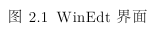
\includegraphics[scale=1]{figures/capnocolon}}}
\subfigure[序号带“:”]{\centering
  \framebox{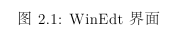
\includegraphics[scale=1]{figures/capcolon}}}
\figcaption{capnocolon选项效果及对比}
\label{pic:capnocolon}
\end{figure}

\begin{figure}
\centering
\subfigure[中文章节编号]{\centering
  \framebox{
\includegraphics[scale=0.52]{figures/titlech}}}
\subfigure[一般编号]{\centering
  \framebox{
\includegraphics[scale=0.505]{figures/titlearbic}}}
\figcaption{titlechinese选项效果及对比}
\label{pic:titlech}
\end{figure}

\section{模板提供的新环境}
模板提供了4个新环境\emph{abstract,cnabstract,thankspage,code}.分别是\emph{英文摘要,中文摘要,致谢,代码}环境,使用方法比较简单,这里不再赘述。

另外,针对数学等需求,定义若干新环境。模板提供的环境见\autoref{tab:env}
\begin{table}
\tabcaption{模板提供的新环境}
\label{tab:env}
\centering
\begin{tabular}{c|c||c|c}
\hline\hline
环境 & 含义 & 环境& 含义\\\hline\hline
abstract&英文摘要&cnabstract&中文摘要\\\hline
thankspage&致谢页&code&代码\\\hline
theorem &定理&lemma &引理  \\\hline
example &例&algorithm &算法  \\\hline
definition &定义  &axiom &公理  \\\hline
property &性质  &proposition &命题 \\\hline
corollary& 推论 &remark &注解  \\\hline
condition &条件  &conclusion &结论  \\\hline
assumption &假设  &prove &证明 \\\hline
proof&证明 &&\\ \hline\hline
\end{tabular}
\end{table}

需要注意的是,这里prove环境翻译为“证明”,事实上,其实prove环境不是用作theorem等类似环境配套证明的,prove环境是与theorem等环境同级别的环境。与theorem等环境相配套的证明环境是proof环境。使用时请注意下两个环境的差异:proof环境是没有编号的,是与theorem这类环境配合使用的;prove环境是有编号的,更多的是类似于证明题的题目。详细的差别见\autoref{pic:proofandprove}。

\begin{figure}
\centering
  \framebox{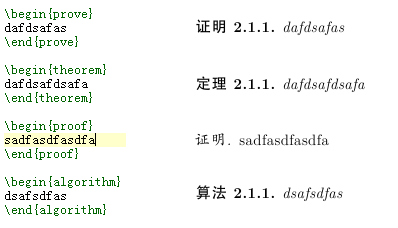
\includegraphics[scale=1]{figures/proofandprove}}
  \figcaption{proof、prove以及部分其他数学环境的差异}
  \label{pic:proofandprove}
\end{figure}


\section{模板提供的新命令}
主要的新命令如下:
\begin{description}
\item[\textbackslash figcaption\{\}]{效果是无论是否在图形环境中均生成图标题}
\item[\textbackslash tabcaption\{\}]{效果是无论是否在表格环境中均生成表标题}
\item[\textbackslash scite\{\}]{效果是得到如\scite{deng:01}这样的参考文献上标引用}
\item[\textbackslash chuhao]{改变字体大小为初号,类似的有\verb|\xiaoyihao|(小一号)直到\verb|\qihao|(七号)}
\item[\textbackslash makecover]{制作封面,供制本厂制作封面使用}
\item[\textbackslash maketitle]{制作扉页,中英文标题在一起}
\item[\textbackslash makeseparatetitle]{制作独立的中英文封面,中英文封面各一张\footnote{对于扉页格式,教务处没有规定,根据喜好二选一即可,或者自行发挥}}
\item[\textbackslash titletail\{\}]{中文标题过长的部分放在这个命令之中}
\item[\textbackslash tutor\{\}]{导师信息}
\item[\textbackslash entitle\{\}]{英文标题}
\item[\textbackslash entutor\{\}]{导师英文信息}
\item[\textbackslash cntime\{\}]{论文完成中文时间,自己填写}
\item[\textbackslash entime\{\}]{论文完成英文时间,自己填写}
\item[\textbackslash department\{\}]{院系中文名称}
\item[\textbackslash No\{\}]{学号}
\item[\textbackslash keywords\{\}]{英文关键字,在英文摘要环境中使用}
\item[\textbackslash cnkeywords\{\}]{中文关键字,在中文摘要环境中使用}
\item[\textbackslash L\{width\}]{表格环境中使用。对表格环境下p{width}命令进行加强,类似的还有C\{width\}和R\{width\}可以在指定宽度的同时指定对齐方式,三个命令分别表示左对齐、居中对齐、右对齐。注意大小写。(范例如下,效果如\autoref{tab:newcmd})}
\end{description}

\begin{minipage}{\textwidth}
\begin{verbatim}
\begin{table}
\tabcaption{几种命令效果对比的对比}
\label{tab:newcmd}
\centering
\begin{tabular}{c||l|c|r|p{2.5cm}|L{2.5cm}|C{2.5cm}|R{2.5cm}}
\hline
命令&l&c&r&p\{width\}&L\{width\}&C\{width\}&R\{width\}\\
\hline
效果&左齐&居中&右齐&定宽&左齐定宽&居中定宽&右齐定宽\\
\hline
\end{tabular}
\end{table}
\end{verbatim}

\tabcaption{几种命令效果对比的对比}
\label{tab:newcmd}
\centering
\begin{tabular}{c||l|c|r|p{2.5cm}|L{2.5cm}|C{2.5cm}|R{2.5cm}}
\hline
命令&l&c&r&p\{width\}&L\{width\}&C\{width\}&R\{width\}\\
\hline
效果&左齐&居中&右齐&定宽&左齐定宽&居中定宽&右齐定宽\\
\hline
\end{tabular}
\end{minipage}


\section{使用模板的一些注意事项}
把题目写在\verb|\title{}|中,只有题目过长的时候,再将过长的部分放在\verb|\titletail{}|中去(如\autoref{pic:title})。 

\begin{figure}
\centering
  \framebox{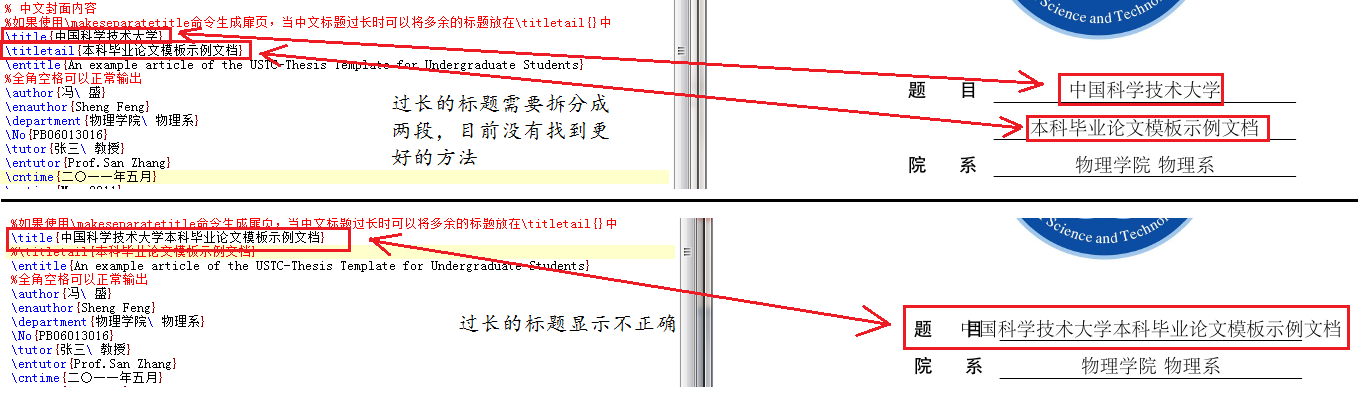
\includegraphics[scale=0.4]{figures/title}}
  \figcaption{过长的标题}
  \label{pic:title}
\end{figure}

比如:

对于短的题目——\\ \rule{4em}{0pt}\textbackslash title\{较短的题目\} 

对于较长的题目——\\\rule{4em}{0pt}\textbackslash title\{较长的题目的前一部分\} 
\\\rule{4em}{0pt}\textbackslash titletail\{较长的题目的后一部分\}

公式、章节、图和表格等(不包括脚注和参考文献)的交叉引用可以使用 \verb|\autoref{label}|来得到正确的引用。例如使用 \verb|\autoref{some_pic}|可以得到“图 X”的引用,使用 \verb|\autoref{some_table}|可以得到“表 X”的引用。

建议使用 \verb|\figcaption{}|命令得到所有图形的标题,表格也是。这样无论是否在图形环境中均能够得到正确的带图/表编号的标题,而在图形环境之外使用 \verb|\caption{}|命令会报错。

封面是按照制本厂的要求制作的,其中行宽和行高都是固定的,中文标题最多占两行,英文标题最多占三行。如果您的题目超过了这个限制,请缩减题目长度,不要擅自修改模板中的相关配置参数。

